%%%%%%%%%%%%%%%%%%%%%%%%%%%%%%%%%%%%%%%%%%%%%%%%%%%%%%%%%%%%%%%%%%%%%
% LaTeX Template: Project Titlepage Modified (v 0.1) by rcx
%
% Original Source: http://www.howtotex.com
% Date: February 2014
% 
% This is a title page template which be used for articles & reports.
% 
% This is the modified version of the original Latex template from
% aforementioned website.
% 
%%%%%%%%%%%%%%%%%%%%%%%%%%%%%%%%%%%%%%%%%%%%%%%%%%%%%%%%%%%%%%%%%%%%%%

\documentclass[12pt]{report}
\usepackage[a4paper]{geometry}
\usepackage[myheadings]{fullpage}
\usepackage{fancyhdr}
\usepackage{lastpage}
\usepackage{biblatex}
\usepackage{url}
\usepackage{hyperref}
\usepackage{graphicx, wrapfig, subcaption, setspace, booktabs}
\usepackage[T1]{fontenc}
\usepackage[font=small, labelfont=bf]{caption}
\usepackage{fourier}
\usepackage[protrusion=true, expansion=true]{microtype}
\usepackage[english]{babel}
\usepackage{sectsty}
\usepackage{url, lipsum}


\newcommand{\HRule}[1]{\rule{\linewidth}{#1}}
\onehalfspacing
\setcounter{tocdepth}{5}
\setcounter{secnumdepth}{5}

%-------------------------------------------------------------------------------
% HEADER & FOOTER
%-------------------------------------------------------------------------------
\pagestyle{fancy}
\fancyhf{}
\setlength\headheight{15pt}
\fancyhead[R]{Center for Urban Science and Progress}
\fancyfoot[R]{Page \thepage\ of \pageref{LastPage}}
%-------------------------------------------------------------------------------
% TITLE PAGE
%-------------------------------------------------------------------------------

\begin{document}

\title{ \normalsize \textsc{Capstone Project for the Master of Science in Applied Urban Science and Informatics}
		\\ [2.0cm]
		\HRule{0.5pt} \\
		\LARGE \textbf{\uppercase{Bus Reliability Metrics using Public MTA Bus Time Data}}
		\HRule{2pt} \\ [0.5cm]
		\normalsize \today %\vspace*{5\baselineskip}
		}

\date{}

		\author{
				Jiaxu Zhou \\
				Yuqiao Cen \\
				Matthew Urbanek \\
				Bonan Yuan \\
				Sara Arango-Franco \\ 
				\\
				Advisors: \\
				Dr. Kaan Ozbay \\
				Dr. Huy T. Vo \\
				\\
				Sponsor Agency:\\
				Department of Transportation, City of New York\\
				\\
		\textbf{Center for Urban Science and Progress} \\
		\textbf{New York University}}
		
	

\maketitle
\tableofcontents
\newpage

%-------------------------------------------------------------------------------
% Section title formatting
\sectionfont{\scshape}
%-------------------------------------------------------------------------------

%-------------------------------------------------------------------------------
% BODY
%-------------------------------------------------------------------------------

\section*{Brief}

Despite a growing demand for public transportation in New York City, bus ridership levels are declining.  This can be explained by drops in vehicle speeds and customer perceptions of dependability.  The \textit{New York City Department of Transportation} (NYC DOT) wished to engage the \textit{New York University Center for Urban Science and Progress} (CUSP) to explore the use of public vehicle location data from the \textit{Metropolitan Transit Authority} (MTA) Bus Time to generate operational data relevant to the DOT's planning decisions.  This information is provided in the form of reliability metrics for bus service.

Based on the MTA \textit{Automated Vehicle Location} (AVL) data and its public Bus Time API, the team performed a data assessment analysis for the data generating process and the data collection process. We also deliver methods for estimating bus travel and stop times, measuring reliability with different metrics, and settles the ground for the DOT to identify the distribution of reliability measurements as a function of factors regarded as relevant to their practice.
        
\section*{Acknowledgements}

We would like to express our sincere appreciation to all who have lent us hands during this time.  First of all, we would like to show our sincere gratitude to our sponsor agency, the New York City Department of Transportation, for giving us an opportunity to focus on this important city issue.  We would specially like to to thank Jeremy Safran, who gave us plenty of insight into the way the DOT wants to treat and understand bus data analytics.  Secondly, we would like to express our gratitude to our advisors, Dr. Kaan Ozbay and Dr. Huy T. Vo., not only for their technical expertise but for their generosity and willingness to lead us through this process.  Invaluable consultation on use of the Bus Time API for performance analysis was provided by Nathan Johnson and Kuan Butts, primary authors of the NYC Bus Transit Data project (http://busdataapi1.cloudapp.net/); and Chris Pangilinan and Zak Accuardi at Transit Center.  Last but not least, we would like to thank Kai Zhao, Abdullah Kurkcu, Ender Morgul, and our classmates in CUSP who gave us assistance and advice during this process.  We will always be thankful.


%-------------------------------------------------------------------------------
% REFERENCES
%-------------------------------------------------------------------------------
\newpage

\section{Overview and background}


\subsection{	Statement and Description}
Although demand for public transportation in New York City is growing, bus ridership levels are declining.  Many reasons can explain this, including drops in vehicle speeds and customer perceptions of dependability.  This project focuses on identifying these two factors along the city's MTA operated bus routes, in the form of reliability metrics that are relevant to the DOT as the municipal traffic authority.

The DOT receives batch files from MTA containing archived basic AVL data, but the agency lacks a formal process for compiling and analysing it according to their decision making capabilities (such as those related with road design and traffic management), which substantially differ from the MTA's purposes and reach.  Additionally, the basic AVL data differs significantly in density and reported elements compared to those from the Bus Time API.  Although the MTA, being the agency in charge of operations, has internally defined metrics used for scheduling, planning and analysis of the bus service, this their attention is on the bus level instead of the whole system level, which is more of the interest of the DOT.
 
To help the DOT improve their planning efficiency, this project aims to assess the usefulness of Bus Time data for measurement of the dependent variable metrics related to bus performance and reliability, enabling the agency to, in a further analysis, understand the effect of independent variables that affect service quality. 

\subsection{Goals}

The goals of the project can be summarized as follows:

\begin{enumerate}
\item Perform a thorough data quality assessment on the MTA Bus Time data.

\item Implement metrics related to the performance of the buses with respect to customer experience, which in part considers their planned schedule.

\item Document the entire process and deliver flexible code, so both data quality assessment and reliability measurements can be reproduced by the agency.
\end{enumerate}

\newpage

\section{Project offerings}

This Capstone project hopes to address the core urban challenge of transportation planning with the following contributions:
\begin{itemize}
\item The conclusion that public, self-service data can be applied to evaluate transit operations performance, independent of the operating agency
\item A framework for a new, more efficient data interface between agencies and for processing of the data
\item Demonstration of the potential for implementation of the framework using only a personal computer and open source software
\item New value realized from a public service originally implemented with a narrower scope in mind
\end{itemize}

\newpage

\section{Approach}

In this section we discuss the data retrieval, processing and reliability measurement techniques.  Because MTA does not continually publish archived AVL data, data was retrieved from the Bus Time API in real-time and stored on NYU CUSP servers.  Parsing is required both to store data efficiently and to decrease processing time of subsequent methods.  We then propose a variety of transit system performance metrics that can be applied using these data before discussing the results.


\subsection{Bus time data extraction}

MTA's AVL data is acquired using a ''get'' request to a \href{http://bustime.mta.info/}{web service} offered by the MTA to the public.  The service uses a standard rotocol, originally developed in Europe, called \textit{Service Interface for Real-Time Information} (SIRI). 

Per MTA's recommendation, the response data is requested in JSON format (\textit{Javascript Object Notation}).  JSON offers a flexible structure, for example allowing elements to be stored in hierarchies, or a combination of named and unnamed elements.  JSON does not transform directly to a tabular layout and as a result cannot be imported by typical data analysis tools like Microsoft Access or Excel without first parsing it.

Parsing can be performed using a variety of approaches.  A small program that can be written on almost any personal computer (a macro, or command-line script) may be acceptable for parsing one JSON response, requiring in the order-of-magnitude one second for each JSON.  However this is likely unacceptable for reading and aggregating any meaningful amount of archived JSON response files (entire days, or entire lines over multiple days).  Advanced techniques requiring additional software or hardware can significantly improve processing time by distributing the data across multiple processing units.  Regardless of the technique, the extracted data has a straightforward structure, containing text and numerical elements (which can be stored as text), appropriate for storage in a comma-separated values (CSV) file.

The SIRI standard calls for date-time representation according to the ISO 8601 standard.  While this can be read directly and used for many typical calculations (for example, elapsed time), it poses a problem when performing any analysis requiring date or time data from the planned schedule for the buses.  Those analysis require both the ''true'' date-time element as well as the trip reference date.  Here are two example comparisons of a bus trip's estimated departure from its first stop and the corresponding scheduled departure time. Such a comparison may be used to explain whether bus reliability can be attributed to operational issues such as late departures from the depot.  Note the conversion and that time zone information is dropped; in the data for this project, both SIRI response and schedule data time elements are written in the local time zone.

\vspace{0.5cm}

\resizebox{\textwidth}{!}{
\begin{tabular}{l l l l}
\hline
trip\_id & Time stamp & Converted time stamp & Scheduled time \\
\hline
OH\_B6\-Weekday\-SDon\-077600\_M101\_100 & 2016\-06\-13T13:09:32.000\-04:00 & 0d\+13:09:32
& 13:08:55 \\
MV\_B6\-Weekday\-SDon\-041500\_M5\_206 & 2016\-06\-14T01:20:42.000\-04:00 & 1d\+01:20:42 &
25:12:15 \\
\hline
\end{tabular}
}

\vspace{0.5cm}


\subsection{Big Data Techniques}

Our data extraction step picks the useful information from the original json and dumps the redundancies. This step shrinks file size by 30 times and facilitates future analysis by creating a  human readable table that can easily be analysed through Excel by anyone.


%\begin{figure}[!ht]
%  \caption{Original sample extraction from DOT.}
%  \centering
%    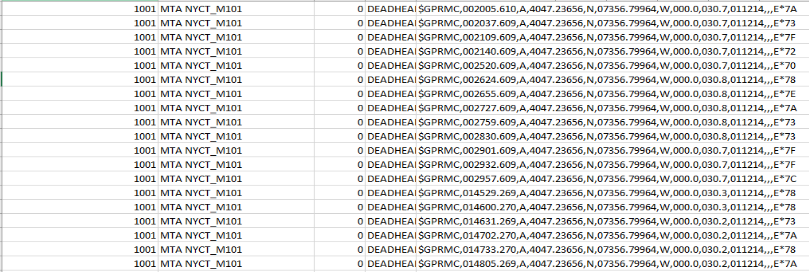
\includegraphics[scale=0.6]{/home/saf537/Documents/CUSP/Capstone/Bus-Capstone/plots/DOT}
%\end{figure}

However, due to the time required to process and parse each JSON, we decided to apply big data techniques for the data. Each JSON file is originally between one and three megabytes, before parsing; the entire set of collected data is about 3 terabytes..We apply Apache Spark along with some Spark SQL techniques for manipulating the data in large scale. It takes around 30 to 45 minutes for the processing the entire year data depending on the performance of the server.  Without the use of this technique, processing only one day of data takes 10 to 15 minutes.

%\begin{figure}[!ht]
%  \caption{Our data extraction using Spark.}
%  \centering
%    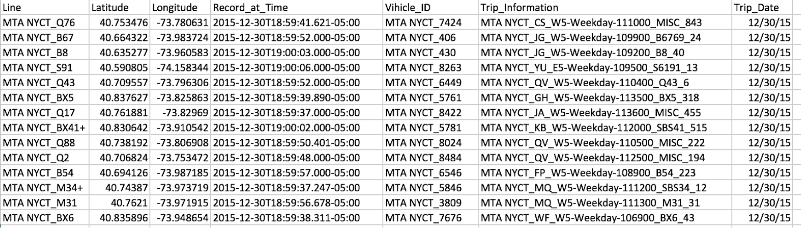
\includegraphics[scale=0.6]{/home/saf537/Documents/CUSP/Capstone/Bus-Capstone/plots/Spark}
%\end{figure}



\resizebox{\textwidth}{!}{
\begin{tabular}[small]{l|l|l}

\textbf{JSON ELEMENT(schema)} & \textbf{Column NAME} & \textbf{Explanation} \\
\hline
\hline
LineRef &	ROUTE\_ID &	Name of bus line(B42) \\
VehicleLocation.Latitude	& latitude	& latitude of record \\
VehicleLocation.Longitude &	longitude	& longitude of record \\
RecordedAtTime & recorded\_time & What time it gets recorded \\
VehicleRef & vehicle\_id & ID of vehicle \\
FramedVehicleJourneyRef.DatedVehicleJourneyRef	& TRIP\_ID & 	Same as trip\_id in GTFS*\\
FramedVehicleJourneyRef.DataFrameRef &	trip\_date	& Date of the trip \\
JourneyPatternRef & SHAPE\_ID	& Same as shape\_id in GTFS* \\
StopPointRef	&STOP\_ID &	Id of next stop,Same as stop\_id in GTFS*\\
Extensions.Distances.DistanceFromCall & distance\_stop & Distance to next stop \\
Extensions. Distances.CallDistanceAlongRoute & distance\_shape & 	Stop\_s total distance along the shape \\
Extensions. Distances.PresentableDistance & status & Report the current status of bus to next stop \footnote{Approaching, at stop, 1 station away.}\\
DestinationRef & destination & Headsign of bus\\


\end{tabular}
}

\subsection{Schedule data extraction}

Schedule data is published by MTA according to the General Transit Feed Specification, a standard established in 2006 and now widely used by transit agencies and developers.  One transit feed is essentially a small relational database, containing a minimum of six tables and any of seven optional tables.  Basic required data in a transit feed file are routes, trips, stops, stop times, and effective date ranges.  MTA does not include optional metadata that can be used to distinguish multiple publications covering the same schedule period.

\subsection{Data quality assessment} 
We implement three general approaches to assessing the completeness and validity of Bus Time data.  Schedule data feeds from MTA are presumed to be complete and accurate, given their widespread use.

\begin{enumerate}
\item Analysis of time-series patterns
\item Correlation of Bus Time data length to planned level of bus activity, as informed by schedule data
\item Validation of individual elements
\end{enumerate}



\subsection{Arrival time estimation techniques}

Three methods are investigated for estimating a vehicle’s arrival time at a certain location, such as a bus stop. Arrival time estimates are the basis for most measurement and identification related to bus reliability, such as running times and headway.  Calculation of headway, which is in turn the basis for many performance metrics, also requires estimates of all vehicles’ arrival times at a certain location. Missing estimates (whether due to the data generating process or the chosen estimation algorithm) must be identified; without them, the resulting headway will be the difference in arrival times of non-sequential vehicles.

The first method is use to use a spatial algorithm to identify any data points within a certain radius of the location, and make an estimation from within that subset. Possible calculations on that subset are to take earliest or latest time recorded, the median time recorded, or apply an interpolation to generate a point-estimate at the exact location. The second method is to apply an interpolation algorithm to all observations reported for a given vehicle’s trip. The tradeoff is that this may be more computation than required if few points along the trip are to be estimated.  The risk Interpolation is that it assumes the bus traveling at uniform speed while in reality the bus speed changes a lot due the complicated traffic condition and traffic lights, especially in New York.

The third method is to apply the interpolation only for stops that are reported in Bus Time as a ''Monitored Call,'' that is, the upcoming stop. The advantage of only interpolating the reported stops is that it avoids the risk of reporting stops that the bus never made (for example, due to a detour) and the risk of high inaccuracy in the event the bus did make the stop (due to the long distance over which times must be interpolated).The tradeoff for the third method is that since many trips are not completely recorded, we may lose a lot of information for the missing part.

\subsection{Reliability metrics}

Wait Assessment is a metric used by New York City Transit, defined in the Transit Capacity and Quality of Service Manual as the percentage of actual headways between successive vehicle arrivals that are less than or equal to a given standard. The wait assessment for bus is only measured on weekdays. It is defined as the percentage of observed service intervals that are no more than the scheduled interval plus 3 minutes during peak (7 a.m. - 9 a.m., 4 p.m. - 7 p.m.) and plus 5 minutes during off-peak (12 a.m - 7 a.m., 9 a.m. - 4 p.m, 7 p.m. - 12 a.m.)

\textit{Wait Assessment} is a simple calculation that can be performed after all headway calculations have been performed for a given location.

\textit{OTP (On Time Performance)} is defined as the positive difference between actual arrival time and schedule arrival time. Different from the measurement of on-time performance percentage by MTA, which is the percentage reflects the number of buses that arrive within a certain time before or after the published schedule, we use the distribution of a group of data to describe the on-time performance for a single trip. The main reason is the criteria is not provided by MTA for buses. However, During low-frequency period, on-time performance is more important while during the high frequency period, the headways matter more. Running Time Adherence (measured in \%) is defined as the average difference between the actual and the scheduled running times relative to the scheduled running time. When the actual running time is shorter than the schedule, the measure is called shorter running time and otherwise longer running time.

Similarly, headway regularity (measured in \%) is defined as the average difference between the actual and the scheduled headways relative to the scheduled headway. The Headway Regularity describes how evenly distributed actual bus is in relation to scheduled service. If two consecutive buses are further from (or closer to) each other than the scheduled headway, the difference is called a longer (or shorter) headway difference. Bus bunching is an extreme example of short headway.

\newpage

\section{Results and implications for practice}

Differences worth noting between the compilation of Bus Time data and DOT's files are listed in Table \ref{diff}. \footnote{Unclear if reported speed is instantaneous or averaged since last transmission.}

\vspace{0.5cm}

\captionof{table}{Differences between DOT and Bus Time data. }
\resizebox{\textwidth}{!}{
\begin{tabular}{l| ll}
\label{diff}
 & \textbf{DOT flat file} & \textbf{Bus Time API} \\
 \hline
Source database & Archived & Real-time \\
Sample frequency & 30 seconds & Limited by reliability of interface (max 30 seconds) \\
Spatiotemporal elements & Raw NMEA, including speed* & Only time and location (projected 
onto shapeline) \\
Trip elements & Route and status only & Includes inferred elements, like Next Stop and Trip ID
\end{tabular}
}








 

\subsection{Data quality assessment}


 In this part, it is trying to find out whether the data are reliable or not. It is a overview of the whole dataset. By visualizing the date, it can find out that whether it is reasonable or not.
 
 \subsubsection*{Missing data}
 
  The first step to figure out the data quality is to know the information that the data contain. By summarizing the data get from all the jsons files by using Spark, it can find that the data cover a total number of 318 different bus lines and 340 days in a year. So though this project tried to focus on the whole year data (from 2015-1-1 to 2015-12-31), there still existed missing data for some days. Here shows all the missing days in \ref{m_days}.
  
  \begin{figure}[!ht]
  \caption{Missing days in the dataset.}
  \label{m_days}
  \centering
    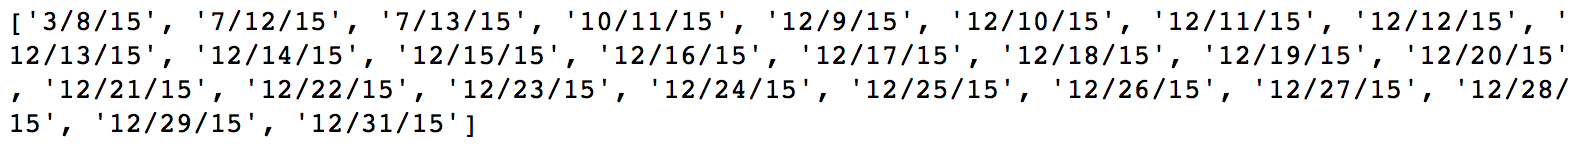
\includegraphics[scale=0.6]{/home/saf537/Documents/CUSP/Capstone/Bus-Capstone/plots/missing_days}
\end{figure}

      From the list of missing days , it can find that December is a month with the most missing data, which contains 21 days without data. So it is necessary to find out what factors cause this problem. If it is caused by some uncontrollable factors such as weather, some mitigation plan could come out. But if it is caused by some human factors of systems factors, it should be avoided in the future.
      
      \subsubsection*{Visualization of records throughout the year}
      
        Here shows the whole year respond record in \ref{m_alldays}.



\begin{figure}[!ht]
  \caption{Bus records count for all days in 2015.}
  \label{m_alldays}
  \centering
    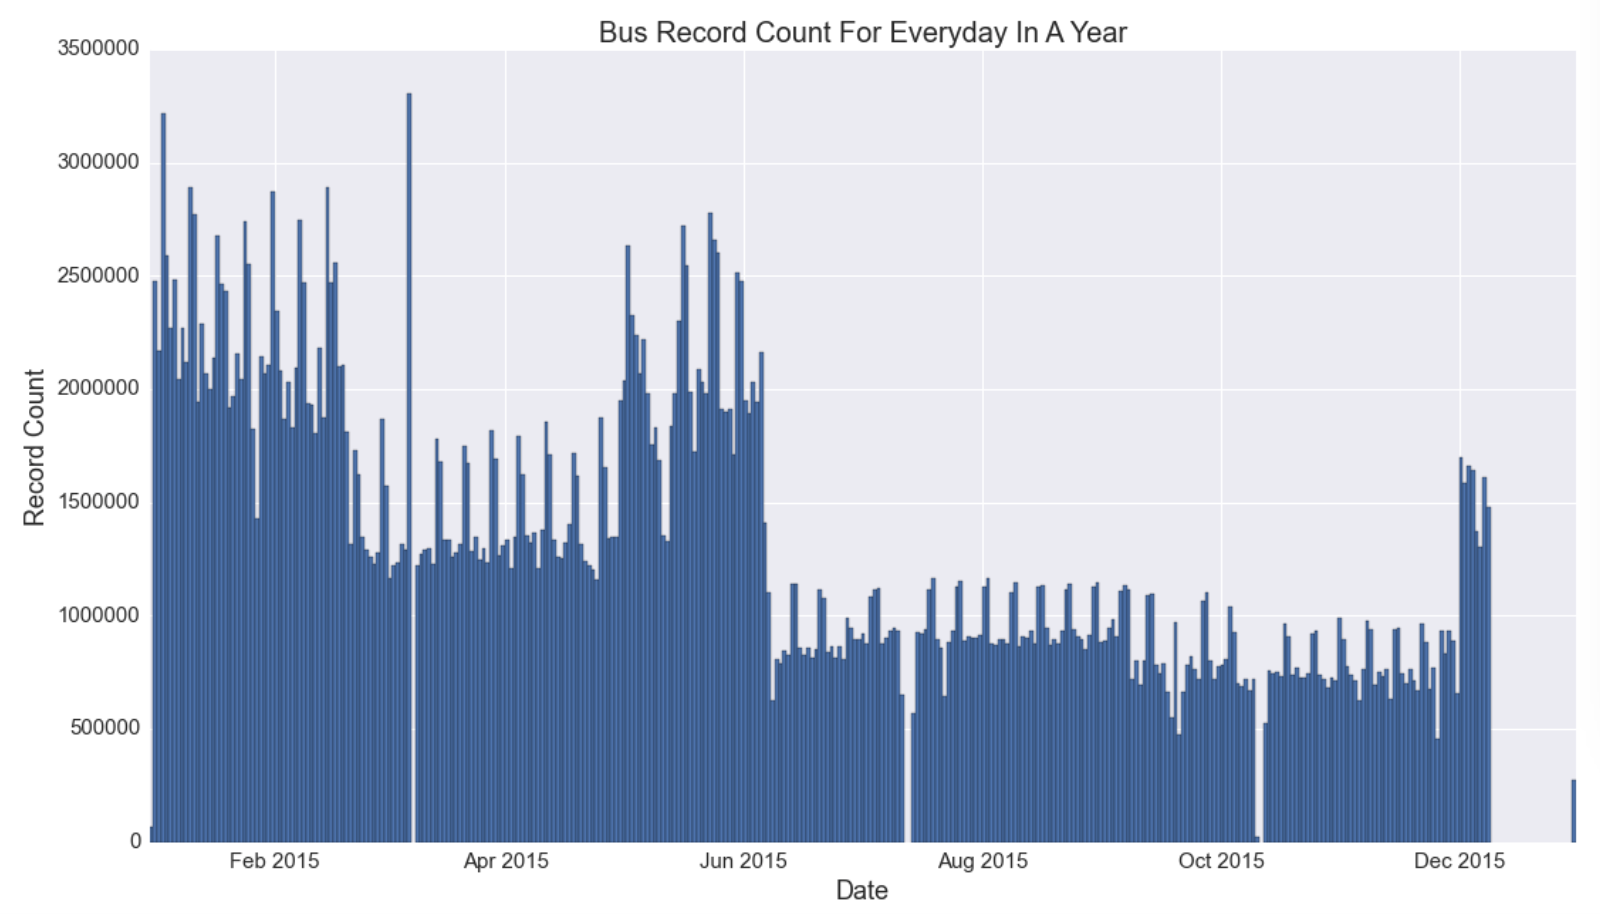
\includegraphics[scale=0.6]{/home/saf537/Documents/CUSP/Capstone/Bus-Capstone/plots/whole_year_record}
\end{figure}

   From the plot, it can find that there are some regularities existing. Normally, seven days is a cycle, and weekdays have less record count than weekends. But January, February and May are not that obvious. And as there are some missing data in December, the regularity in December is not obvious. 
      There exist four obvious change in this plot. The first one is in February, second in May, third in June, and the last one in December. It may exist some factors that affect these change. Further analysis is needed to find out these factors and could help with the bus schedule planning.
      Also, it can find that March 7th has an extremely high record but March 8th is a day without data which do not exist in other missing days. It can infer that there exist some possibility that data for March 8th may merge with March 7th.
      
      \subsubsection*{Daily response records}
      
       Here shows the everyday respond record in \ref{week}.

\begin{figure}[!ht]
	\label{week}
  \caption{Bus records count for day of the week in 2015.}
  \centering
    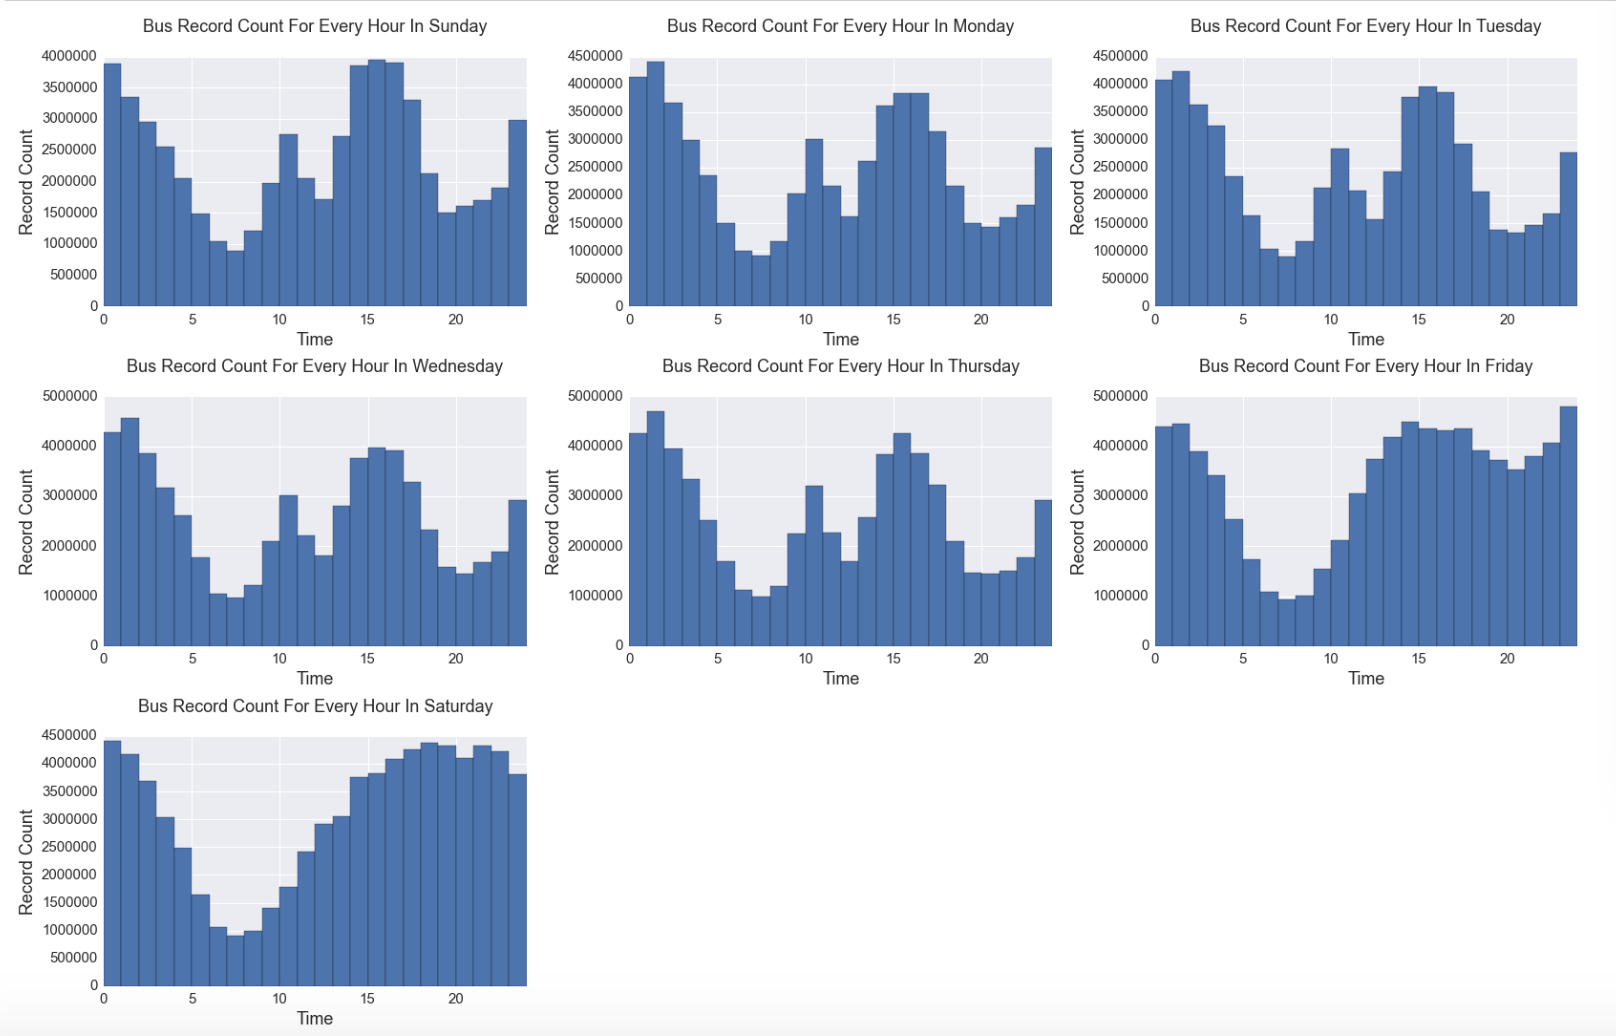
\includegraphics[scale=0.6]{/home/saf537/Documents/CUSP/Capstone/Bus-Capstone/plots/whole_day_record}
\end{figure}

   From the plot, it can find that weekdays have the same trend and weekends has the same trend. In weekdays, 9am to 11am would exist another peak in a day. And after 5pm, bus records declines regularly. It is reasonable because 9am to 11am and 5pm are the rush hours in a day. And in weekends, after 8am, bus records increase regularly.
      Based on the visualization of the bus records for everyday and for every hour in a day, it can find that the data are quite reasonable and the further analysis based on these data would be reliable. 
      
      \subsubsection*{Gaps (time dimension)}
      
        As the bus is transmitting every 30 seconds, for the first part of gaps analysis, it find out which hour in a day has the least 30-second interval. Here shows the 30-second interval distribution for a day in \ref{week_day}.

\begin{figure}[!ht]
\label{week_day}
  \caption{Bus records count for day of the week in 2015.}
  \centering
    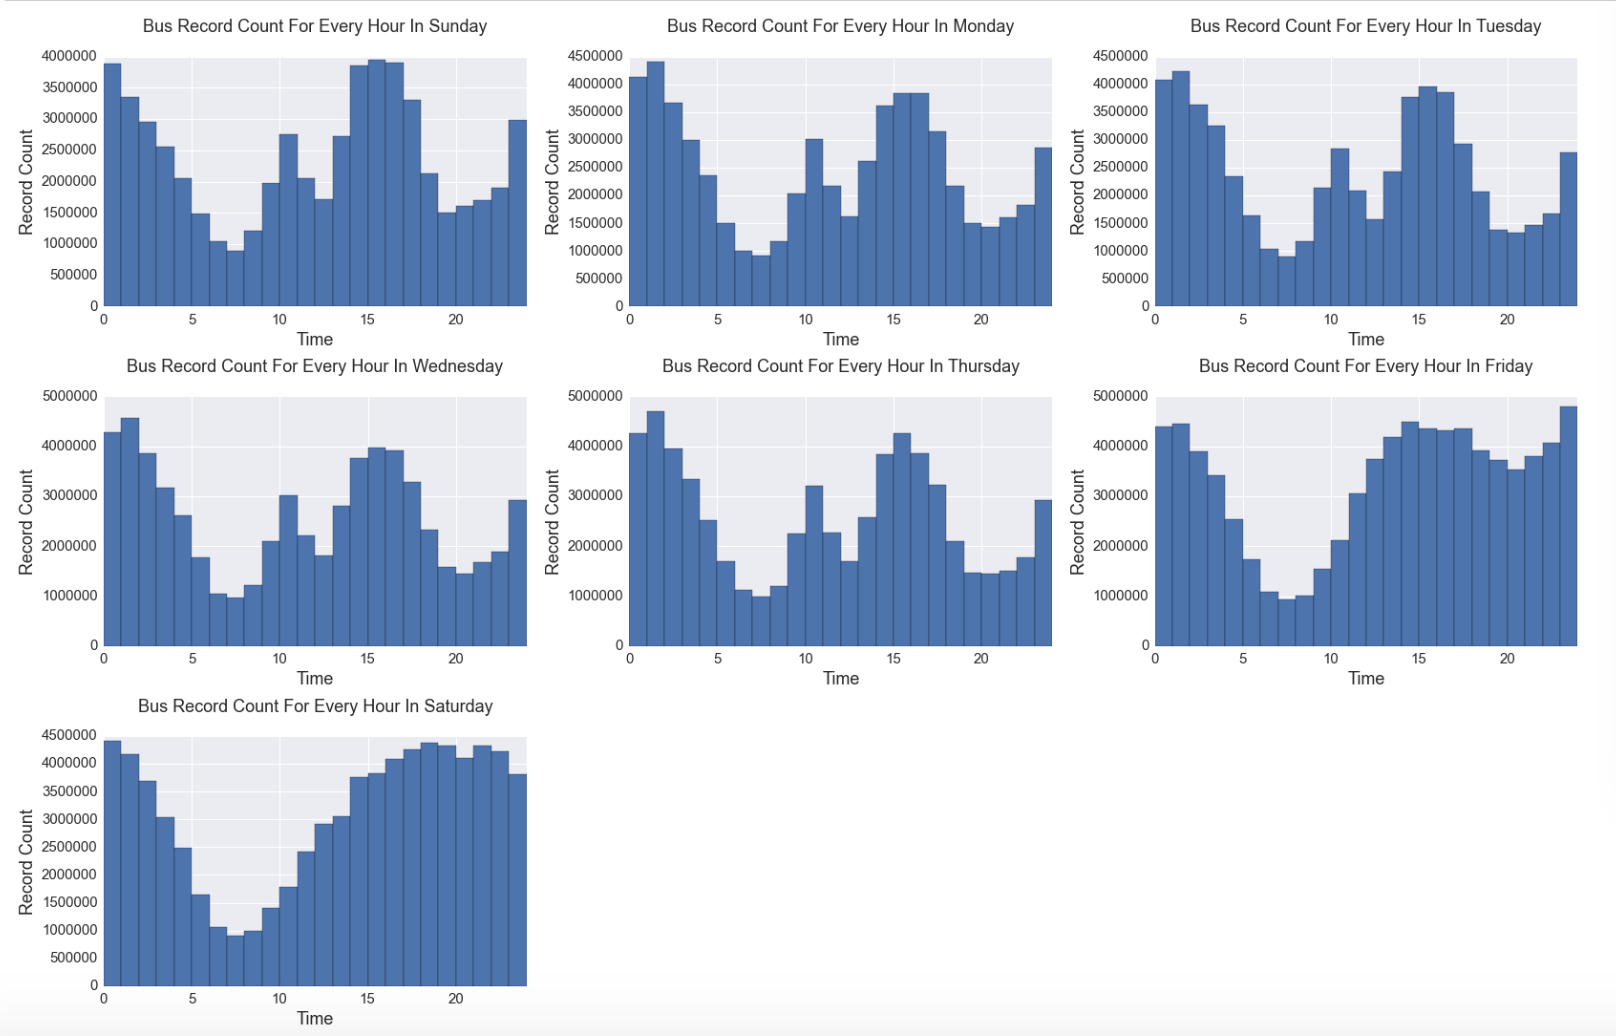
\includegraphics[scale=0.6]{/home/saf537/Documents/CUSP/Capstone/Bus-Capstone/plots/whole_day_record}
\end{figure}


 From the plots, it can found that 9 a.m. is the time that has the least bus respond record  interval within 30 seconds. That may exist some gap in 9 a.m. So for further analysis, it may be valuable to compare the data with GTFS data. This shows the focuses of future gap analysis and an example of the comparison between AVL data and GTFS data.




\begin{figure}[!ht]
  \caption{Bad: Major gaps without data for most vehicles, over several hours (2015-01-06).}
  \centering
    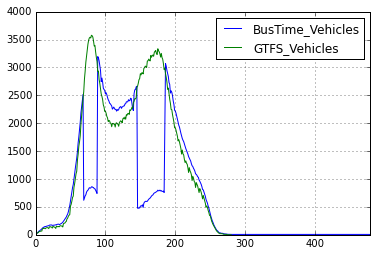
\includegraphics[scale=0.6]{/home/saf537/Documents/CUSP/Capstone/Bus-Capstone/plots/trip_coverage_20150106}
\end{figure}


\begin{figure}[!ht]
  \caption{Less Bad: Shorter gap (<1 hour) with no data from some vehicles (2015-11-01).}
  \centering
    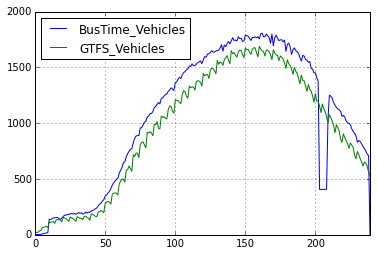
\includegraphics[scale=0.6]{/home/saf537/Documents/CUSP/Capstone/Bus-Capstone/plots/trip_coverage_20151101}
\end{figure}


\begin{figure}[!ht]
  \caption{Good: No significant gaps in API performance (2015-12-03)}
  \centering
    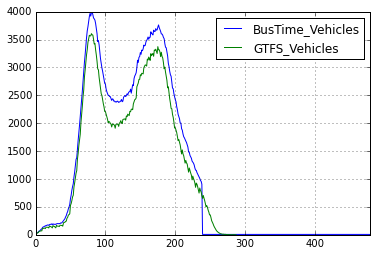
\includegraphics[scale=0.6]{/home/saf537/Documents/CUSP/Capstone/Bus-Capstone/plots/trip_coverage_20151203}
\end{figure}


\subsection{Demonstrations of the methods applied to the dataset}

The practices of transportation planning and analysis rely heavily on vehicle arrival-time data.  The first phase of this report explained the retrieval of real-time Automated Vehicle Location data and application of methods for estimating those arrival times in actual operations.  The following list demonstrates some typical analytic techniques and discusses their validity when applying these data, given the known limitations to its density and accuracy.  Included are data of arrival times from the schedule, published in the widely-adopted General Transit Feed Specification, but discussion of its data generation process is not in scope.  Generally, many high-level performance metrics are simple ratios expressing the proportion of events (such as a vehicle arrival, or completed trip) that meet some criteria (such as arriving within 5 minutes of its scheduled time).  The problem with these binary measurements is that the methods ignore the shape (defined in mathematics as higher moments) of a distribution - for example, a "long tail," or if the distribution is multi-modal.

\begin{itemize}
\item \textbf{Distribution of headway}: In higher-frequency transit routes, arrivals are considered reliable when the headway is more consistent and closer to customers' expectation.  (The ideal distribution is 100\% density at the expected value, that is, no deviation.  Our definition of Headway Adherence is binary and allows for some deviation).  The distribution of headway for a less-than-reliable service is not always a normal bell-curve.  This is because of the tendency for delayed buses to become even more delayed, as the larger number of waiting passengers increases dwell times, which in turn reduces overall travel speed.  When bunching occurs, the headways of the "bunched" buses (i.e., those that closely follow a preceding delayed bus) approach zero, while there is no theoretical upper limit for the headway of the delayed bus.
\item \textbf{Bunching rate}: Variations in dwell time and variations between-stop travel time related to traffic and operator behavior are the major causes of vehicle bunching along a route (Gellei 2010).  Measurement of dwell time and travel time will be discussed later in this section.  The resulting bunching condition can be measured.  For this analysis, we consider the bunching condition to occur when headway is less than one minute.  The bunching ratio is the percentage, at a certain stop, of arrivals under bunching condition compared to total vehicle arrivals.  This is very similar to Headway Adherence except that it measures the tail of the distribution, not the middle.  Bunching ratio can be calculated and compared for a variety of stops and routes, as shown in \ref{bunch}.


\begin{figure}[!ht]
  \caption{Headway Bunching Rate at Stops for Three Brooklyn Bus Routes.}
  \label{bunch}
  \centering
    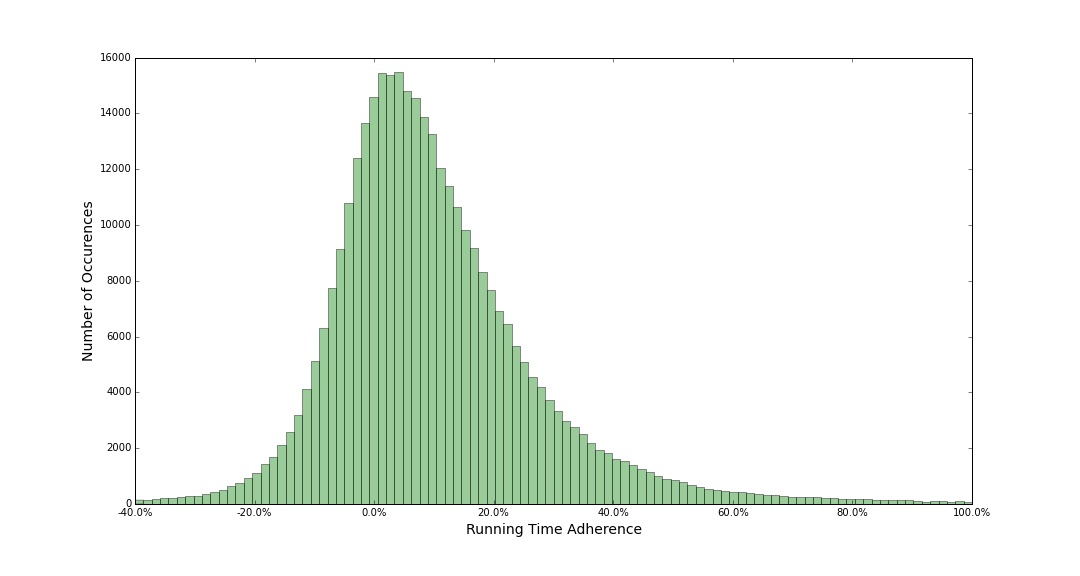
\includegraphics[scale=0.4]{/home/saf537/Documents/CUSP/Capstone/Bus-Capstone/plots/running_time_adherence}
\end{figure}



\item \textbf{Distribution of running time adherence:} Best practice in schedule planning is to forecast running time using historical data, but exclude outliers.  An outlier often represents an occurrence of some enroute incident (such as a police action or a parade) and should not be factored into planning a typical-day bus schedule. Outliers skew upward the distribution of actual running times, since there is a physical upper limit to the vehicle's speed, but no limit to the number and severity of enroute incidents. Because the schedules are created based on historical distributions excluding outliers, the resulting error, defined as running time variance, will tend to be positive. The error can be mitigated by artificially increasing the planned running time (for example, by including the outliers, or adding some arbitrary value), but it is generally not cost-effective to do so, or impacts the reliability of subsequent trips operated by the same vehicle or operator. 


One example descriptive analysis is to plot the distribution of normalized running time variances. Visible in this example, \ref{adh}, is both the central tendency -- slightly positive -- and the wide spread of the distribution, indicating very inconsistent running time adherence.  Strategies to reduce the inconsistency are not in the scope of this project.




\begin{figure}[!ht]
  \caption{Running time adherence.}
  \label{adh}
  \centering
    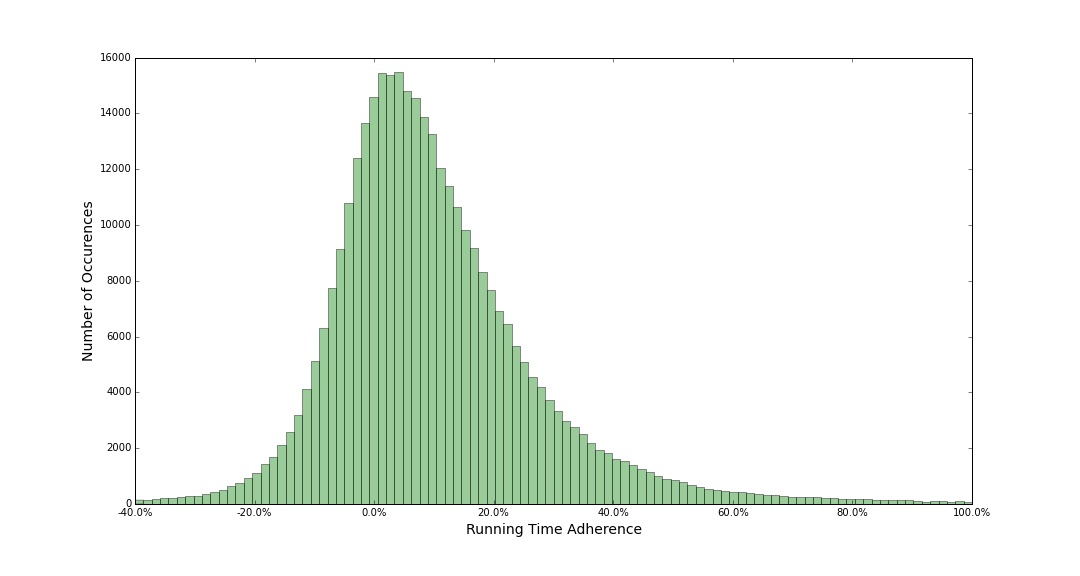
\includegraphics[scale=0.4]{/home/saf537/Documents/CUSP/Capstone/Bus-Capstone/plots/running_time_adherence}
\end{figure}


\item \textbf{Performance with respect to vehicle distance along route:} It is generally accepted in the theory of urban public transportation that longer routes have worse reliability, as defined by the metrics discussed so far.  Another analytic technique is to plot one of the metrics for a given route (or, more specifically - one shape variation of a route).  \ref{ols} is the summary of an ordinary least squares (OLS) regression, taking Wait Assessment as the dependent variable and the vehicle's progression along the shape (in terms of number of stops made) as the independent variable.  The resulting parameter value has strong statistical significance, rejecting the null hypothesis that route length has no relationship to performance.  The example in \ref{wastop} both supports that conclusion and suggests which segments along the route contribute most to the decline.

%\begin{figure}[!ht]
%  \caption{Correlation of Wait Assessment and Stop Sequence Number.}
%  \label{ols}
%  \centering
%    \includegraphics[scale=0.4]{/home/saf537/Documents/CUSP/Capstone/Bus-Capstone/plots/OLS Regression Results}
%\end{figure}


\begin{figure}[!ht]
  \caption{Average Wait Assessment by Stop Sequence Number, Route B41.}
  \label{wastop}
  \centering
    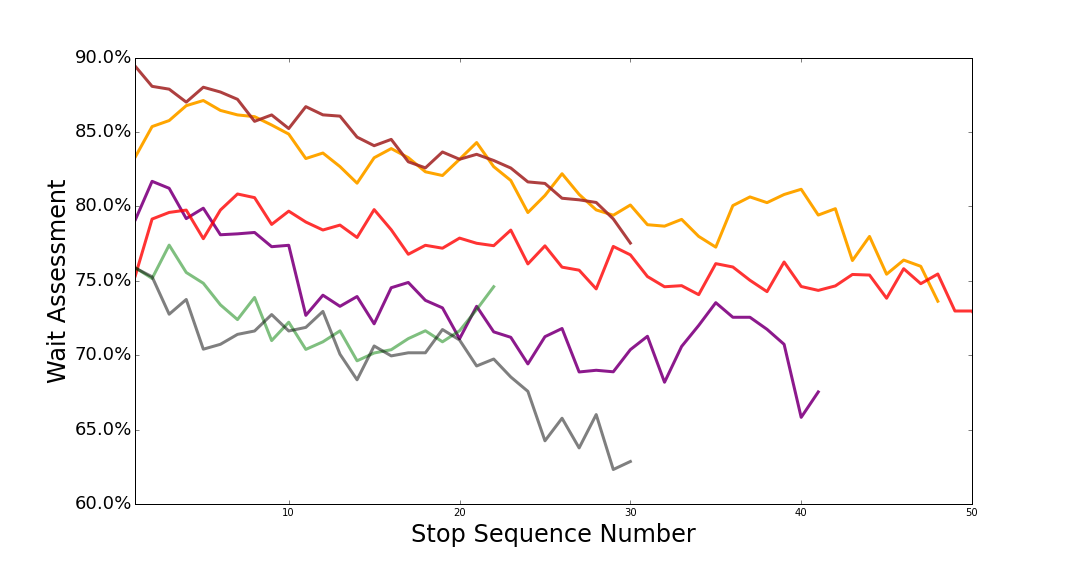
\includegraphics[scale=0.4]{/home/saf537/Documents/CUSP/Capstone/Bus-Capstone/plots/wa_by_stop_sequence}
\end{figure}

\item \textbf{Spatial distribution of travel speeds:} Because Bus Time records contain discrete time and location, speed calculations are difference-based averages, not instantaneous (or quasi-instantaneous) samples.  The other challenge in descriptive statistics about speed at fixed location(s) is that the sequential observation points of multiple vehicles are not aligned; for example it is extremely unlikely that multiple vehicles record the "ping" from exactly 100 meters and again at exactly 200 meters along a route-shape.  However re-sampling is possible if mean speeds are treated as continuous curves with respect to distance.  The new distribution at a point is defined as the collection of mean speeds of all vehicles passing that point.  \ref{msd} demonstrates the changing moments of the distribution over the length of a route-shape, along with grid lines indicating the stop locations.

\begin{center}
\begin{figure}[!ht]
  \caption{Moving speed distribution.}
  \label{msd}
  \centering
    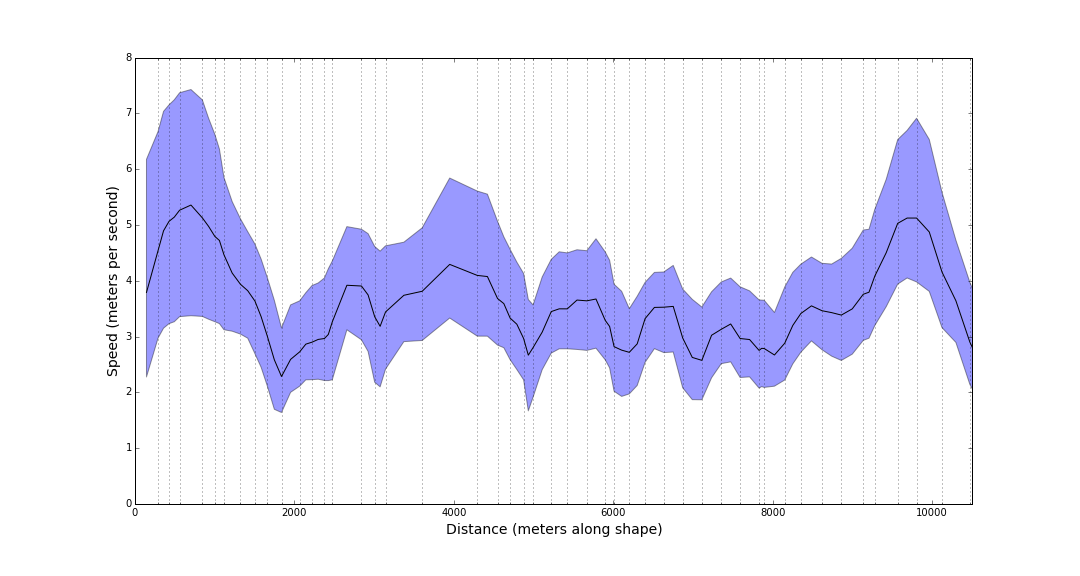
\includegraphics[scale=0.45]{/home/saf537/Documents/CUSP/Capstone/Bus-Capstone/plots/moving_speed_distribution}
\end{figure}
\end{center}

\item \textbf{Spatial distribution of slow/stopped condition} - A list of slow/stopped events can be created by identifying the beginning and end location and times for each occurrence of the condition.  Naturally, many of these events will be at stop locations.   That subset of the slow/stopped events may theoretically support analysis of dwell time, however even when using data having the maximum density possible according the data generation process (every 30 seconds), analysis of dwell time at individual stops is not possible; previous research suggests that the majority of stops have dwell time of less than 30 seconds (Pangilinan 2011).  The remaining subset are slow/stopped events not occurring at stop locations.  High spatial density of these events indicates a recurring problem with traffic flow, which in turn increases travel time and contributes to occurrence of bunching condition.  (In order to exclude the normal interaction with traffic signals, the events can be filtered to only include those above some minimum, related to traffic signal cycle lengths).

Figure \ref{adh} shows the estimated percentage of vehicles in slow/stopped condition and many points along a route-shape.  While some extreme values are apparent, they are generally at stop locations and the variance of the remaining points is minimal, even at other stop locations.  This suggests that the density of the data may be insufficient to identify .



\begin{figure}[!ht]
  \caption{Moving speed distribution.}
  \label{adh}
  \centering
    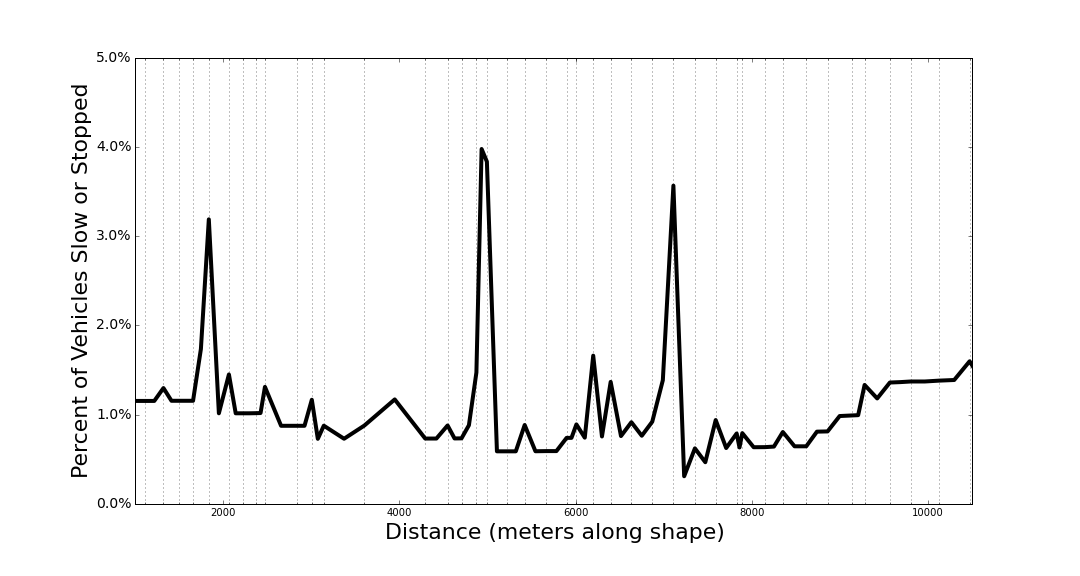
\includegraphics[scale=0.4]{/home/saf537/Documents/CUSP/Capstone/Bus-Capstone/plots/percent_vehicles_slow_or_stopped}
\end{figure}




\end{itemize}


\subsection{More discussion on the approach}

The main risk identified by our approach is reproducibility in terms of data fetching and of framework dependency. Our data feed depends on a public API that is always subject to interruptions, and the Big Data processing requires the HDFS management system and Spark. It may take time and computational and technical resources to handle them, and deprecation is always a hazard. Despite of this, those potential sources of failure have been proven to be increasing in robustness and trustworthiness during the last years.

The main advantages of our approach rely on the fact that it is based on open source software (such as Python, HDFS and Spark) with a wide and increasing support community around them, but also on the fact that our code is simple to share and reproduce. Since Big Data software is relatively new, we kept most of the data manipulation in simple SQL or Python scripts, which is specially convenient for the client.

The biggest challenge for our approach to be implemented in practice by cities is that of processing large amounts of raw data into information because it requires big data techniques for anything beyond small samples (i.e. one line, one day, etc.). Even processed datasets being structured can demand more than what can be offered by single/dual core applications. Data supporting higher-level analysis techniques can be managed with any off-the-shelf database system, including sqLite (open source SQL) or even a series of CSVs.

It is worth noting that, while the MTA does not publish archived Bus Time data (except for a sample in 2014), we are providing the code for anybody to collect it, and this is an important step that must be kept into account when discussing about Privacy.  Besides this, the Vehicle ID field is not anonymized, so the contributions of our project are subject to have unlikely yet feasible implications regarding Privacy.

\subsection{Conclusions and future work}

\subsubsection*{Conclusions}


This project studies the bus performance in New York City and its correlation metrics based on the GPS data offered by MTA. The MTA bus GPS database collects the location of each bus every 30 seconds. After estimating the departure and arrival time for each bus at each stop, we use measurement like headways and wait assessment to figure out the bus performance and reliability. Taking one-year data as our object of study, the data is extremely huge so that big data techniques (mainly Spark) are widely used in this project. In order to make our work easy to share and reproduce, we choose to use the SQL API to decide on the parsing of the data, which enables the DOT to easily make changes by editing the SQL script. 

Positive aspects of our approach include the fact that we focused this analysis on the viewpoint of the DOT; the fact that we were able to successfully process large volumes of data; the fact that we identified pitfalls and challenges of using the MTA Bus Time data for the purposes of the agency (as it was requested from us) and the fact that we enable a flexible implementation of different methods to estimate times and locations, as well as to measure schedule-reliability performance.

Potential pitfalls and areas of improvement are the fact that we used formal metrics that were not tailored for the DOT nor New York City, and the abundance of assumptions that inevitably scale up in the form of measurement errors.

Influence: Similar methodologies and concepts could be used in other cities and traffic models. The big data technology applied in not only traffic analysis but also city wide urban issue offers more reliable results compared with traditional sample studies.  


\subsubsection*{Future work}

\begin{itemize}
\item Inference study of the effect of several traffic or design conditions on reliability.
\item Improve the current visualization tool, and adapt it to be responsive and interactive to different queries.
\item Have a more detailed work flow including our code, to be easily implemented into every day tasks in the DOT.
\item Further optimize the algorithms hereby used for the Big Data portion of the work.
\item Further Applications
\begin{itemize}
\item Other cities (need to pay attention to data structure, bus GPS data in some cities collect departure and arrival time instead of location).
\item Other traffic modes (eg. Subway, city bike. Need to pay attention to the different features of each kinds of traffic mode).
\end{itemize}
\end{itemize}



\newpage
\appendix
\section*{\\Sample visualizations} \label{App:AppendixA}


\begin{figure}[!ht]
  \caption{On time performance aggregated by stop over 2015.}
  \centering
    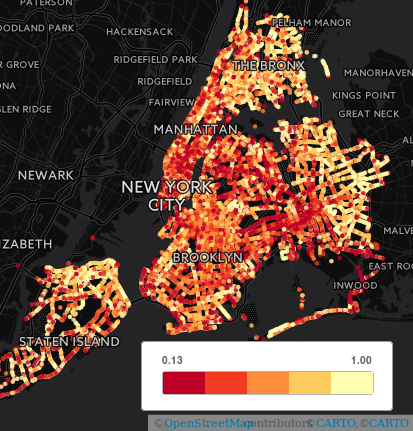
\includegraphics[scale=0.8]{/home/saf537/Documents/CUSP/Capstone/Bus-Capstone/plots/on_time_performance_stops}
\end{figure}

\newpage
\section*{\\Sample results} \label{App:AppendixB}

\captionof{table}{Sample result metrics file (headshot example).}
\resizebox{\textwidth}{!}{
\begin{tabular}{|l|c|c|c|c|c|}
\hline
route id & stop id &	date & On Time Performance &	Peak Wait Assessment	& Off-Peak Wait Assessment \\
\hline
Q07 & 350232 & 1/2/2015 &	0.831395 & 	0.891566 &	1  \\
Q25 & 550032 & 1/2/2015 & 0.720737 &	0.72388 &	0.760368 \\
Q34	& 501132 & 1/30/2015 & 0.666667 & 0.910714 & 0.918699 \\
\hline
\end{tabular}
}

\vspace{1cm}

The fields \textit{Running time adherence}, \textit{Headway regularity} and \textit{Excess wait time} remain to be calculated and added to the schema.

\begin{thebibliography}{14}

\bibitem{Lin}
W. H. Lin and J. Zeng, "An experimental study of real-time bus arrival time prediction with GPS data," Transp. Res. Rec., no. 1666, pp. 101- 109, Jan. 1999.

\bibitem{Raj}
Rajat Rajbhandari, Steven I. Chien, and Janice R. Daniel, ''Estimation of bus dwell times with APC information'', Transportation Research Record 1841 Paper No. 03- 2675, 2003.

\bibitem{Min-Tang}
Min-Tang Li, Fang Zhao, Lee-Fang Chow, Haitao Zhang, and Shi-Chiang Li, ''Simulation Model for Estimating Bus Dwell Time by Simultaneously Considering Numbers of Disembarking and Boarding Passengers'', Transportation Research Record 1971, 2006.

\bibitem{Fazhi}
LI Fazhi, Yang Dongyuan, and Ma Kai, ''Bus Rapid Transit (BRT) Bunching Analysis With Massive GPS Data,'' National Science and Technology Support Program of China (NO. 2009BAG17B01), 2013.

\bibitem{Levine}
Brian Levine, Alex Lu, and Alla Reddy, ''Measuring Subway Service Performance at New York City Transit: A Case Study Using Automated Train Supervision (ATS) Track-Occupancy Data,'' TRB 2013 Annual Meeting, 2013.

\bibitem{DanWan}
Dan Wan, Camille Kamga, Jun Liu, Aaron Sugiura, and Eric B. Beaton, ''Rider perception of a ‘light’ Bus Rapid Transit system - The New York City Select Bus Service,'' Transport Policy 49 (2016) 41–55, Apr. 2016.

\bibitem{Bie}

Yiming Bie, Xiaolin Gong, and Zhiyuan Liu, ''Time of day intervals partition for bus schedule using GPS data,'' Transportation Research Part C 60, pp. 443–456, Sep. 2015.

\bibitem{Safran}
Jeremy S. Safran, Eric B. Beaton, and Robert Thompson, ''Factors Contributing to Bus Lane Obstruction and Usage in NYC: Does Design Matter?'' TRB 2014 Annual Meeting, 2014

\bibitem{Pangil}
Christopher Pangilinan, Nigel Wilson, and Angela Moore, ''Bus Supervision Deployment Strategies and Use of Real-Time Automatic
Vehicle Location for Improved Bus Service Reliability,'' Transportation Research Record: Journal of the Transportation Research Board, No. 2063, Transportation Research Board of the National Academies, Washington, D.C., 2008, pp. 28–33. DOI: 10.3141/2063-04.

\bibitem{Yang}
Yingxiang Yang, David Gerstle, Peter Widhalm, and Dietmar Bauer, ''The Potential of Low-Frequency AVL Data for the Monitoring and Control of Bus Performance,'' TRB 2013 Annual Meeting, 2013.

\bibitem{ShiAn}
Shi An, Xinming Zhang and Jian Wang, ''Finding Causes of Irregular Headways Integrating Data Mining and AHP,'' ISPRS Int. J. Geo-Inf. 2015, 4, 2604-2618; DOI:10.3390/ijgi4042604, Nov. 2015.

\bibitem{Jinil}
Jinil Chang, Mohamad Tala, and Satya Muthuswamy, ''A Simple Methodology To Estimate Queue Lengths at Signalized Intersections Using Detector Data,'' TRB 2013 Annual Meeting, 2013.

\bibitem{Chris}
Christopher Pangilinan and Kristen Carnarius, ''Traffic Signal Timing for Optimal Transit Progression in Downtown San Francisco,'' San Francisco Municipal Transportation Agency, San Francisco, CA, 2011.

\bibitem{Reed}
Simon Reed, ''Transport for London - Using Tools, Analytics and Data to Inform Passengers,'' JOURNEYS, September 2013. \url{https://www.lta.gov.sg/ltaacademy/doc/13Sep096-Reed_TfL-InformPassengers.pdf, accessed 20 Jul 2016.}





\end{thebibliography}

\end{document}

%-------------------------------------------------------------------------------
% SNIPPETS
%-------------------------------------------------------------------------------

%\begin{figure}[!ht]
%	\centering
%	\includegraphics[width=0.8\textwidth]{file_name}
%	\caption{}
%	\centering
%	\label{label:file_name}
%\end{figure}

%\begin{figure}[!ht]
%	\centering
%	\includegraphics[width=0.8\textwidth]{graph}
%	\caption{Blood pressure ranges and associated level of hypertension (American Heart Association, 2013).}
%	\centering
%	\label{label:graph}
%\end{figure}

%\begin{wrapfigure}{r}{0.30\textwidth}
%	\vspace{-40pt}
%	\begin{center}
%		\includegraphics[width=0.29\textwidth]{file_name}
%	\end{center}
%	\vspace{-20pt}
%	\caption{}
%	\label{label:file_name}
%\end{wrapfigure}

%\begin{wrapfigure}{r}{0.45\textwidth}
%	\begin{center}
%		\includegraphics[width=0.29\textwidth]{manometer}
%	\end{center}
%	\caption{Aneroid sphygmomanometer with stethoscope (Medicalexpo, 2012).}
%	\label{label:manometer}
%\end{wrapfigure}

%\begin{table}[!ht]\footnotesize
%	\centering
%	\begin{tabular}{cccccc}
%	\toprule
%	\multicolumn{2}{c} {Pearson's correlation test} & \multicolumn{4}{c} {Independent t-test} \\
%	\midrule	
%	\multicolumn{2}{c} {Gender} & \multicolumn{2}{c} {Activity level} & \multicolumn{2}{c} {Gender} \\
%	\midrule
%	Males & Females & 1st level & 6th level & Males & Females \\
%	\midrule
%	\multicolumn{2}{c} {BMI vs. SP} & \multicolumn{2}{c} {Systolic pressure} & \multicolumn{2}{c} {Systolic Pressure} \\
%	\multicolumn{2}{c} {BMI vs. DP} & \multicolumn{2}{c} {Diastolic pressure} & \multicolumn{2}{c} {Diastolic pressure} \\
%	\multicolumn{2}{c} {BMI vs. MAP} & \multicolumn{2}{c} {MAP} & \multicolumn{2}{c} {MAP} \\
%	\multicolumn{2}{c} {W:H ratio vs. SP} & \multicolumn{2}{c} {BMI} & \multicolumn{2}{c} {BMI} \\
%	\multicolumn{2}{c} {W:H ratio vs. DP} & \multicolumn{2}{c} {W:H ratio} & \multicolumn{2}{c} {W:H ratio} \\
%	\multicolumn{2}{c} {W:H ratio vs. MAP} & \multicolumn{2}{c} {\% Body fat} & \multicolumn{2}{c} {\% Body fat} \\
%	\multicolumn{2}{c} {} & \multicolumn{2}{c} {Height} & \multicolumn{2}{c} {Height} \\
%	\multicolumn{2}{c} {} & \multicolumn{2}{c} {Weight} & \multicolumn{2}{c} {Weight} \\
%	\multicolumn{2}{c} {} & \multicolumn{2}{c} {Heart rate} & \multicolumn{2}{c} {Heart rate} \\
%	\bottomrule
%	\end{tabular}
%	\caption{Parameters that were analysed and related statistical test performed for current study. BMI - body mass index; SP - systolic pressure; DP - diastolic pressure; MAP - mean arterial pressure; W:H ratio - waist to hip ratio.}
%	\label{label:tests}
%\end{table}